\section{Analisi del problema}

A seguito dell'identificazione dei requisiti e dei casi d'uso,
l'analisi del problema entra nel merito del comportamento dell'applicazione,
evidenziandone il rapporto con le funzionalità.
Determina quindi l'architettura logica, che delinea le relazioni fondamentali del sistema,
individuando i componenti logici principali e le loro responsabilità.\\

\subsection{Analisi delle funzionalità}

Le funzionalità vengono dedotte dai casi d'uso,
sintetizzando i servizi principali dell'applicazione.
In particolare, le funzionalità vengono rilevate in base alla loro relazione con i casi d'uso,
alla specificità del compito che assolvono e alla pertinenza reciproca.\\
\\
Si riportano in tabella le funzionalità che racchiudono altri casi d'uso.\\
In particolare, VisualizzaEvento permette di accedere alla maggior parte delle azioni
che l'utente può attuare sugli eventi.
Allo stesso modo GestioneGruppi e GestioneProfili
permettono di eseguire le azioni correlate al loro contesto.\\

\begin{longtable} {|P{7.3cm}|P{8cm}|}
    \hline
    \textbf{Funzionalità} & \textbf{Scomposizione}                                                                                                                            \\
    \hline
    \endhead
    EventiConfermati      & VisualizzaEvento                                                                                                                                  \\
    \hline
    EventiProposti        & VisualizzaEvento                                                                                                                                  \\
    \hline
    VisualizzaEvento      & CreaEvento, ModificaEvento, ConfermaEvento, DisdiciEvento, CondividiConLink, CondividiAiGruppi, CaricaImmagini, EliminaImmagini, ConfermaImmagini \\
    \hline
    GestioneGruppi        & CercaProfili, AggiungiProfiloAlGruppo, CreaGruppo                                                                                                 \\
    \hline
    CercaProfili          & AggiungiProfilo                                                                                                                                   \\
    \hline
    GestioneProfili       & CambiaProfilo                                                                                                                                     \\
    \hline
    \caption{Scomposizione delle funzionalità}
\end{longtable}

\clearpage

Di ogni funzionalità vengono evidenziati il grado di complessità,
la tipologia di azione che svolgono e i requisiti collegati.
Il grado di complessità riassume la quantità e la difficoltà implementativa
delle azioni che una funzionalità ricopre.
La tipologia riporta in maniera generale la qualità dei servizi offerti.
Infine si riportano gli identificatori dei requisiti funzionali che ogni funzionalità soddisfa.\\
\\
A parte il Login, la Registrazione e  ScritturaLog,
il cui servizio è diretto e uniforme in tutta l'applicazione,
tutte le altre funzionalità prevedono una gestione e manipolazione di più dati,
a volte in strutture complicate,
a volte permettendo una modifica puntuale delle informazioni interessate.


\begin{longtable}{|P{3.8cm}|P{4.5cm}|P{2.5cm}|P{4cm}|}
    \hline
    \textbf{Funzionalità} & \textbf{Tipo}                                                 & \textbf{Grado di complessità} & \textbf{Requisiti Collegati}                    \\
    \hline
    Login                 & Interazione esterno e lettura dati                            & semplice                      & R2F                                             \\
    \hline
    Registrazione         & Interazione esterno e memorizzazione dati                     & semplice                      & R1F                                             \\
    \hline
    EventiConfermati      & Interazione esterno e gestione dati                           & complessa                     & R3F, R8F                                        \\
    \hline
    EventiProposti        & Interazione esterno e gestione dati                           & complessa                     & R4F, R9F                                        \\
    \hline
    GestioneGruppi        & Interazione esterno e gestione dati                           & complessa                     & R15F, R16F                                      \\
    \hline
    GestioneProfili       & Interazione esterno e gestione dati                           & complessa                     & R17F, R18F, R19F                                \\
    \hline
    VisualizzaEvento      & Interazione esterno e gestione, lettura e memorizzazione dati & complessa                     & R5F, R6F, R7F, R8F, R9F, R10F, R11F, R12F, R14F \\
    \hline
    AggiornaEvento        & Gestione dati                                                 & complessa                     & R20F                                            \\
    \hline
    RecuperaImmagini      & Lettura dati                                                  & complessa                     & R13F                                            \\
    \hline
    ScritturaLog          & Memorizzazione dati                                           & semplice                      & R21F                                            \\
    \hline
    \caption{Funzionalità}
\end{longtable}

Si procede analizzando i dati che ogni funzionalità gestisce,
indicandone la tipologia, la protezione richiesta e i vincoli correlati,
per conoscere in maniera definitiva tutte le caratteristiche delle informazioni scambiate.
L'analisi delle informazioni non viene riportata in quanto poco rilevante ai fini della tesi,
ma eventuali dettagli saranno riportati quando necessario.\\
\\
A seguito dell'analisi delle informazioni, si procede con l'analisi dei vincoli,
in cui si chiarificano i requisiti non funzionali,
evidenziandone le criticità e quali componenti ne vengono coinvolti.\\


\begin{longtable} {|P{3.5cm}|P{2cm}|P{3.5cm}|P{6cm}|}
    \hline
    \textbf{Requisito}                  & \textbf{Categorie} & \textbf{Impatto}                                                         & \textbf{Funzionalità}                                                                                                                       \\
    \hline
    \endhead
    Semplicità dell'interfaccia         & Usabilità          & Intuitività di utilizzo                                                  & Login, Registrazione, EventiConfermati, EventiProposti, GestioneGruppi, GestioneProfili, VisualizzaEvento, RecuperaImmagini                 \\
    \hline
    Velocità della ricerca dei dati     & Tempo di Risposta  & Maggiore reattività                                                      & EventiConfermati, EventiProposti, GestioneGruppi, GestioneProfili, RecuperaImmagini                                                         \\
    \hline
    Velocità di memorizzazione dei dati & Tempo di Risposta  & Maggiore reattività                                                      & Registrazione, AggiornaEvento, RecuperaImmagini                                                                                             \\
    \hline
    Controllo Accessi                   & Sicurezza          & Peggiorano tempo di risposta e usabilità, migliorano la privacy dei dati & EventiConfermati, EventiProposti, GestioneGruppi, GestioneProfili, VisualizzaEvento                                                         \\
    \hline
    Protezione dei\linebreak Dati       & Sicurezza          & Peggiorano tempo di risposta, migliorano la privacy dei dati             & Login, Registrazione, EventiConfermati, EventiProposti, GestioneGruppi, GestioneProfili, VisualizzaEvento, AggiornaEvento, RecuperaImmagini \\
    \hline
    Scalabilità delle richieste         & Tempo di Risposta  & Minor degradamento delle prestazioni                                     & EventiConfermati, EventiProposti, AggiornaEvento, RecuperaImmagini                                                                          \\
    \hline
    \caption{Analisi dei vincoli}
\end{longtable}


Infine si definiscono logicamente le maschere,
ovvero i componenti visuali essenziali del programma.
A ogni maschera corrisponderà un'interfaccia grafica
attraverso la quale l'utente potrà accedere alle funzionalità.
Vengono quindi associate le maschere alle funzionalità di cui permettono l'esecuzione,
indicando le informazioni relative.\\
\\

\begin{longtable} {|P{4.5cm}|P{6.5cm}|P{4cm}|}
    \hline
    \textbf{Maschera}     & \textbf{Informazioni}                                                                                                               & \textbf{Funzionalità}                     \\
    \hline
    \endhead
    View Login            & email, password                                                                                                                     & Login                                     \\
    \hline
    View Registrazione    & email, password                                                                                                                     & Registrazione                             \\
    \hline
    View EventiConfermati & lista eventi confermati                                                                                                             & EventiConfermati, AggiornaEvento          \\
    \hline
    View EventiProposti   & lista eventi proposti                                                                                                               & EventiProposti, \linebreak AggiornaEvento \\
    \hline
    View VisualizzaEvento & Identificativo utente, titolo, descrizione, data e orario di inizio, data e orario di fine, confermato, immagini, profili associati & VisualizzaEvento, RecuperaImmagini        \\
    \hline
    View GestioneGruppi   & lista gruppi                                                                                                                        & GestioneGruppi                            \\
    \hline
    View CercaProfili     & tag di ricerca, lista profili                                                                                                       & CercaProfili                              \\
    \hline
    View GestioneProfili  & Lista profili, Identificativo utente, Identificativo profilo corrente                                                               & GestioneProfili                           \\
    \hline
    \caption{Maschere}
\end{longtable}

\clearpage




\subsection{Ideazione dell'architettura logica}
Definite le relazioni e le informazioni relative alle funzionalità,
si esprimono logicamente i componenti principali del sistema e le loro relazioni.
Le funzionalità vengono espresse a livello logico tramite package e diagrammi delle classi,
mentre i dati vengono descritti all'interno del dominio. \\
\\
Il modello del dominio individua le entità che rappresentano logicamente le dipendenze tra i dati.
Ogni entità presenta i suoi dati tramite proprietà,
identificate da un nome e dalla tipologia del dato.
Inoltre, all'interno del modello vengono indicati i rapporti tra le entità specificando le cardinalità reciproche.\\
\\
Il dominio di Wyd si concentra attorno a due entità principali: Event e Profile.\\
Gli Event contengono tutti i dati generali degli eventi,
quali l'ora d'inizio e l'ora di fine, il titolo e la descrizione.
Strettamente correlate a loro ci sono le immagini, identificate con Photo.
Ogni Event può avere più Photo, ma una Photo può essere relativa da un solo Event.
I Profile racchiudono i dati dei profili, 
che devono essere identificati da un Tag unico in tutto il programma.
Group rappresenta un gruppo.
Più Profile possono fare parte di un Group ma, 
allo stesso modo, un Profile può appartenere a più Group.\\
\\
L'Account memorizza le informazioni attraverso cui l'utente può accedere e
agire in quanto User, entità che descrive l'utente.
L'utente ha diverse modalità di accesso,
ed è per questo motivo che più Account possono essere relativi allo stesso User.
Lo stesso utente può impersonare più profili,
e un profilo può essere gestito da più utenti.
User e Profile sono quindi connessi in una relazione molti a molti.\\
\\
La maggior parte delle operazioni avrà a che fare con le due entità principali,
da cui l'importanza dell'elemento che ne descrive la relazione, ovvero ProfileEvent.\\
ProfileEvent ha un ruolo centrale in quanto sarà l'unità interrogata
sia quando si vorranno ottenere gli eventi di un determinato profilo,
sia quando bisognerà recuperare i profili relativi a un evento.
Contiene tutte le informazioni relative al particolare profilo sul determinato evento,
rendendolo infatti l'entità più modificata di tutto il progetto.\\
\\

\begin{figure}[h!]
    \begin{center}
        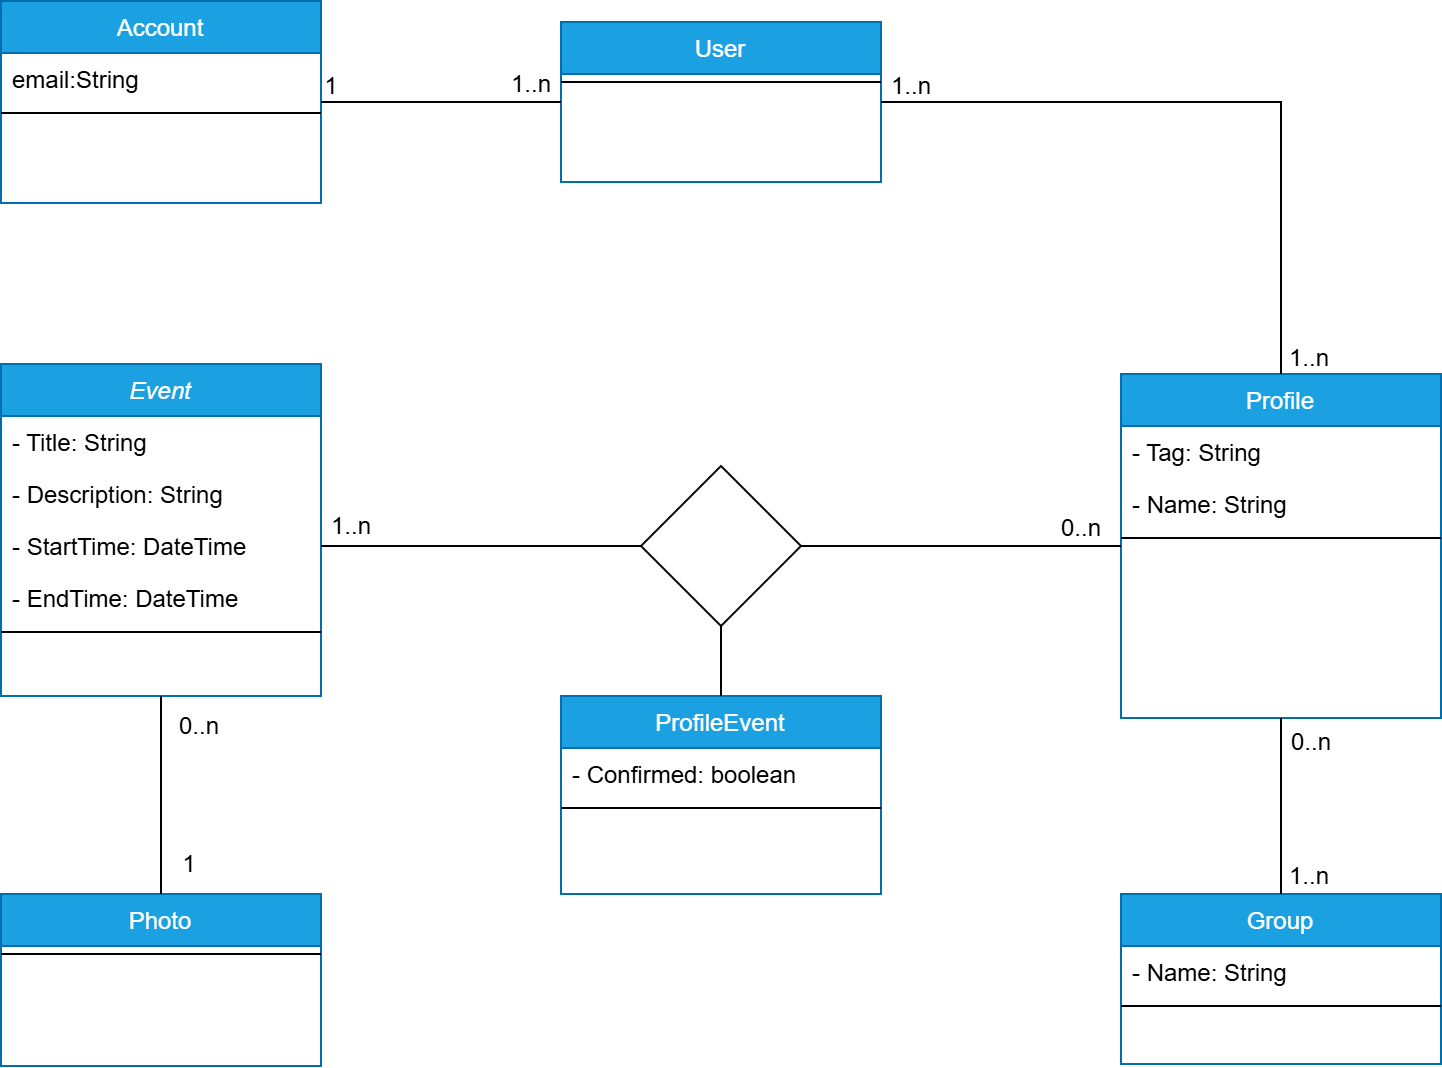
\includegraphics[width=\textwidth]{ModelloDominio.png}
        \caption{Modello del dominio}
    \end{center}
\end{figure}

Il diagramma dei package descrive la divisione delle responsabilità logiche.\\
Ogni package rappresenta una parte di prodotto che soddisfa una determinata responsabilità.
La responsabilità viene individuata in base alla peculiarità e
alle dipendenze delle funzionalità che ricopre.
Si possono così distinguere, ad esempio, package relativi a interfacce grafiche, logiche applicative o gestione della persistenza,
in base alle caratteristiche specifiche del prodotto.
Il diagramma dei package offre una prima struttura delle parti del progetto e del loro rapporto.\\
\\
Distinguiamo i diversi package in base al loro scopo.\\
InterfacciaAccesso e InterfacciaUtente sono le parti che si occuperanno dell'interazione grafica con l'utente.
InterfacciaAccesso deve presentare le schermate di login e di registrazione,
e tutti i passaggi intermedi che saranno necessari.
InterfacciaUtente si occuperà di mostrare le viste per interagire con il resto delle funzionalità dell'applicazione.\\
\\
Il package del Dominio contiene la persistenza principale del progetto,
con tutti i dati delle entità del dominio.
Il package delle Immagini contiene i file multimediali,
recuperabili tramite i metadati salvati sul Dominio.
Il package Log riceve e salva le informazioni relative alle richieste svolte dai vari servizi.\\
\\
GestioneAccesso segue la logica per autenticare gli utenti,
collaborando con InterfacciaAccesso e il Dominio,
per indirizzare l'utente a InterfacciaUtente in caso di login positivo.
GestioneProfilo è il package che racchiude le funzionalità applicative del progetto.
Si occupa quindi d'implementare tutta la logica relativa agli eventi, ai profili e alle loro interazioni.
GestioneAggiornamenti si occupa infine di connettere GestioneProfilo e InterfacciaUtente
per trasmettere le modifiche in tempo reale.\\

\begin{figure}[h!]
    \begin{center}
        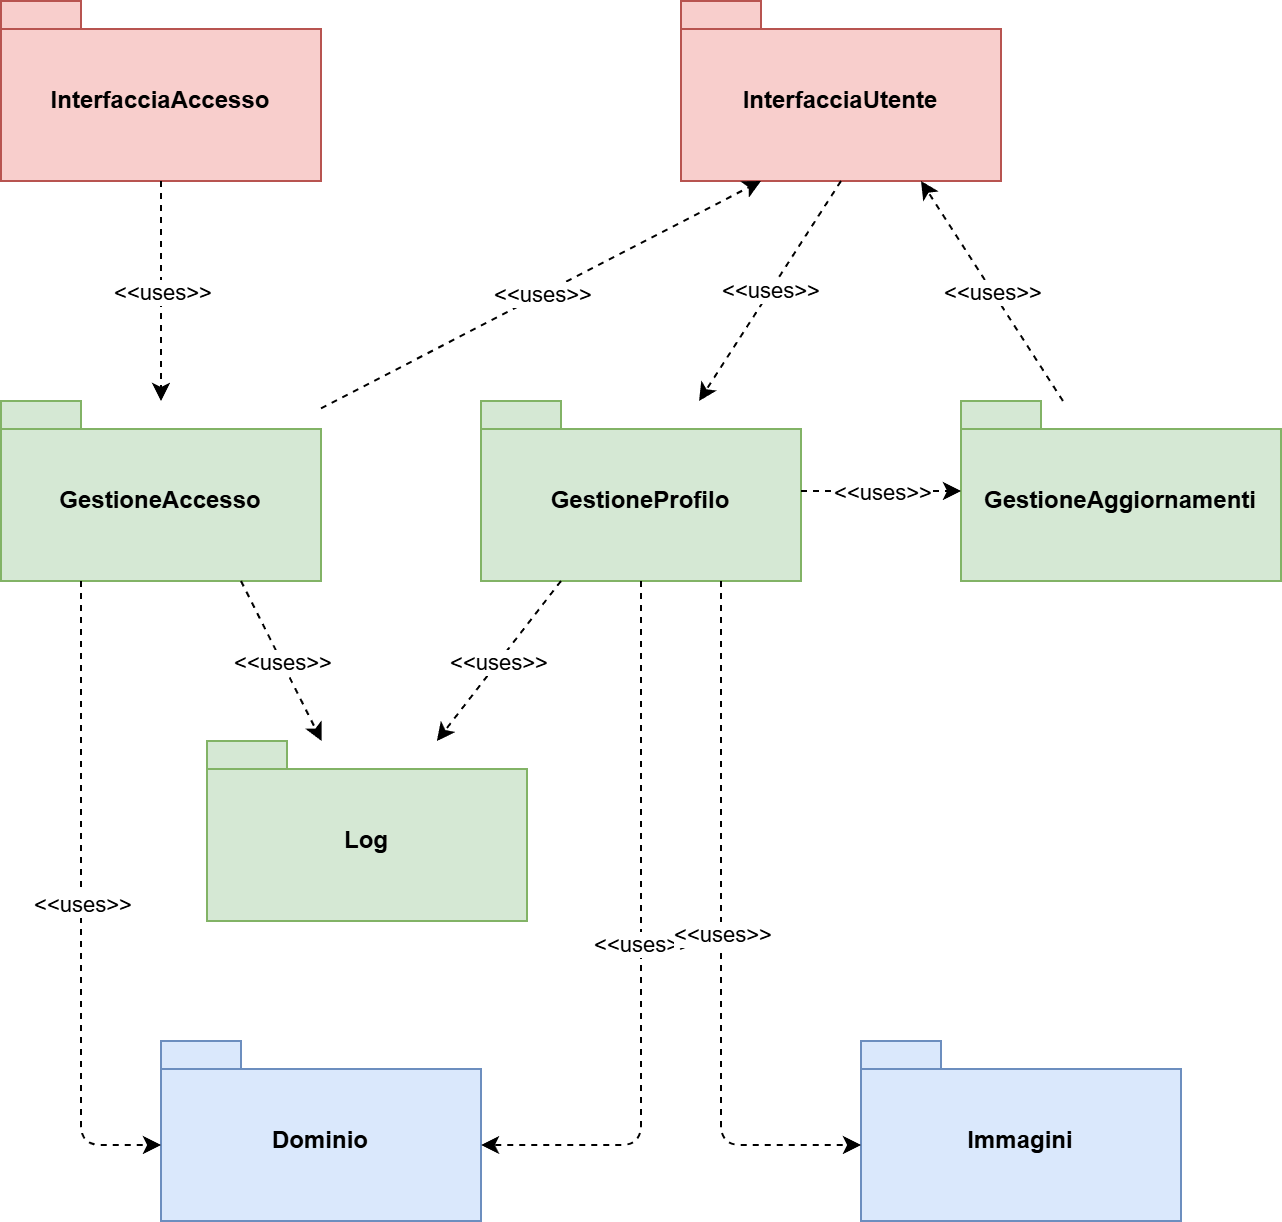
\includegraphics[height=0.5\textheight]{DiagrammaPackage.png}
        \caption{Diagramma dei Package}
    \end{center}
\end{figure}
\clearpage

Ogni package contiene una o più classi che lo implementano.\\
Ogni classe rappresenta un componente logico che assume uno specifico scopo.
Le classi possono presentare dei metodi, ovvero delle istanze che descrivono le funzionalità fornite,
alle quali altri componenti possono fare richiesta di esecuzione.
La definizione delle classi permette di creare una struttura iniziale
presentando le funzionalità minime e le dipendenze tra le parti.\\
\\
InterfacciaUtente ha una classe per ogni funzionalità principale.
Ci sono quindi le classi di ViewEventiConfermati e ViewEventiProposti,
che permettono di visualizzare i relativi impegni.
Attraverso queste interfacce si può interagire con ViewVisualizzaEvento,
per interagire con i dettagli dell'evento.
ViewGestioneGruppi presenta la lista dei gruppi con le azioni relative
e permette l'accesso a ViewCercaProfili,
la schermata per trovare altri profili all'interno dell'applicazione.
ViewGestioneProfili è la classe che visualizza i profili dell'utente e ne permette il cambio.\\

\begin{figure}[h!]
    \begin{center}
        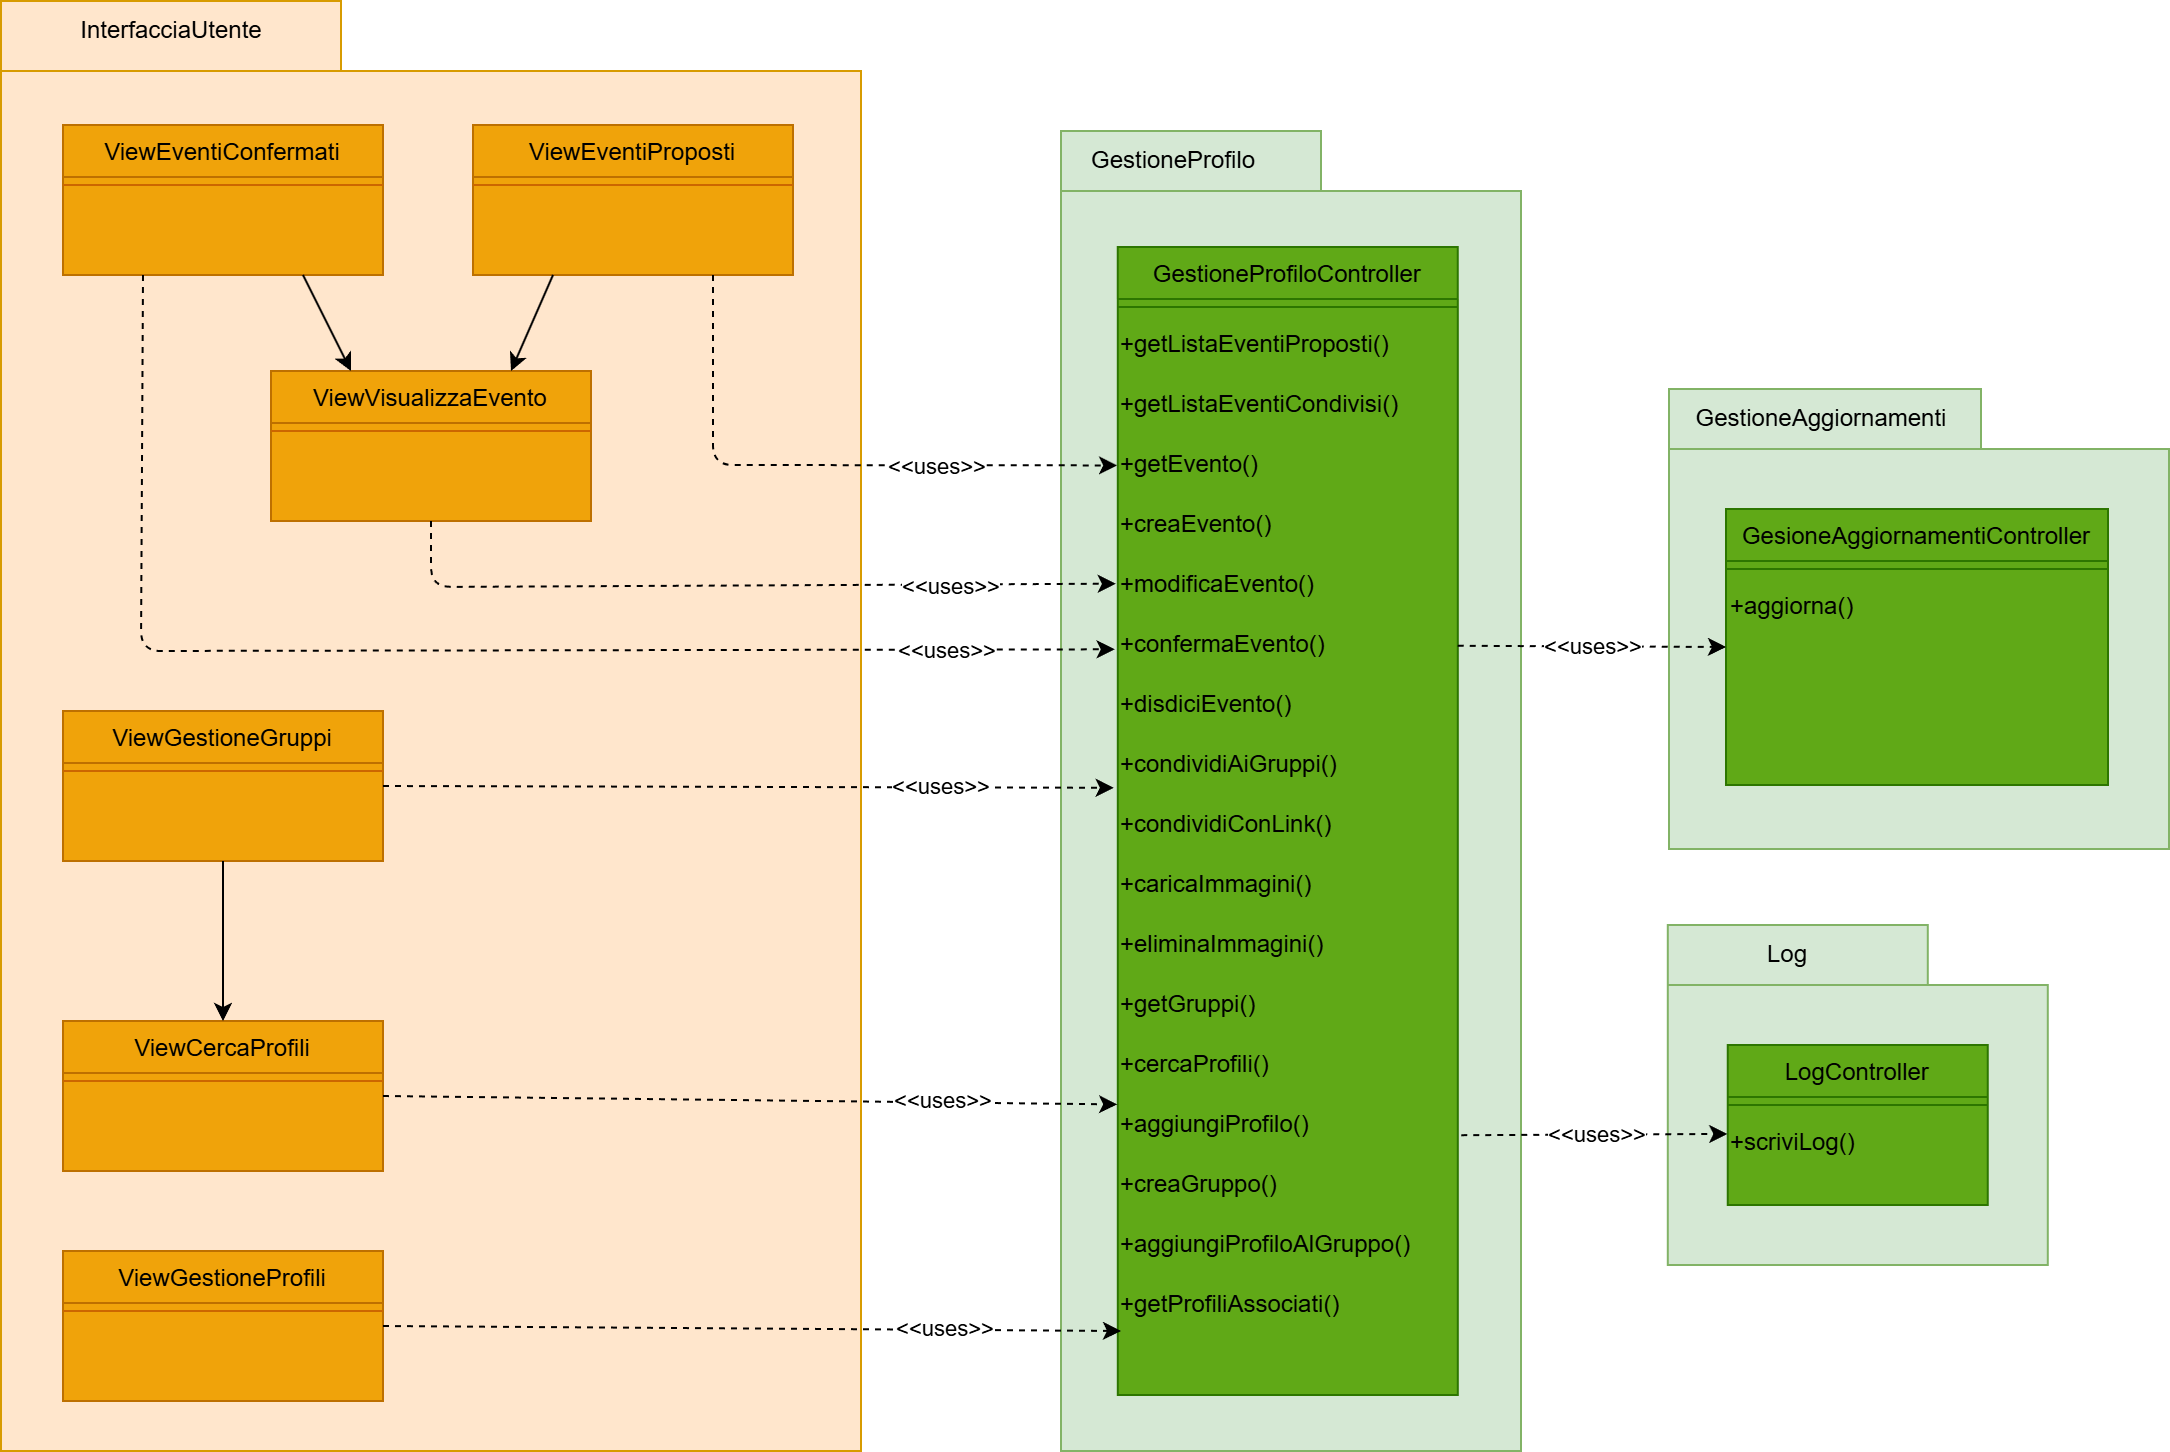
\includegraphics[height=0.46\textheight]{GestioneProfilo.png}
        \caption{Diagramma delle classi: interfaccia utente, gestione profilo e aggiornamenti}
    \end{center}
\end{figure}

GestioneProfilo è il package principale,
a cui le classi di InterfacciaUtente si rivolgono soddisfare le richieste dell'utente.
Prevede una sola classe, GestioneProfiloController,
che risponde alle azioni a cui un profilo può avere accesso, ovvero tutte quelle previste.
Contiene quindi le funzioni relative ai principali casi d'uso,
quali a l'ottenimento degli impegni, la creazione o la conferma dell'evento o il caricamento delle immagini.\\
\\
GestioneAggiornamenti ha il solo compito di aggiornare i dispositivi a seguito di una chiamata da GestioneProfilo,
per cui contiene una classe con un metodo.
InterfacciaAccesso prevede invece due classi, una per il Login e una per la Registrazione.
GestioneAccesso ha una sola classe ma che presenta, seguendo la stessa logica, due metodi distinti.
Il package Log, fornendo un solo metodo, contiene usa sola classe.\\
\\
\begin{figure}[h!]
    \begin{center}
        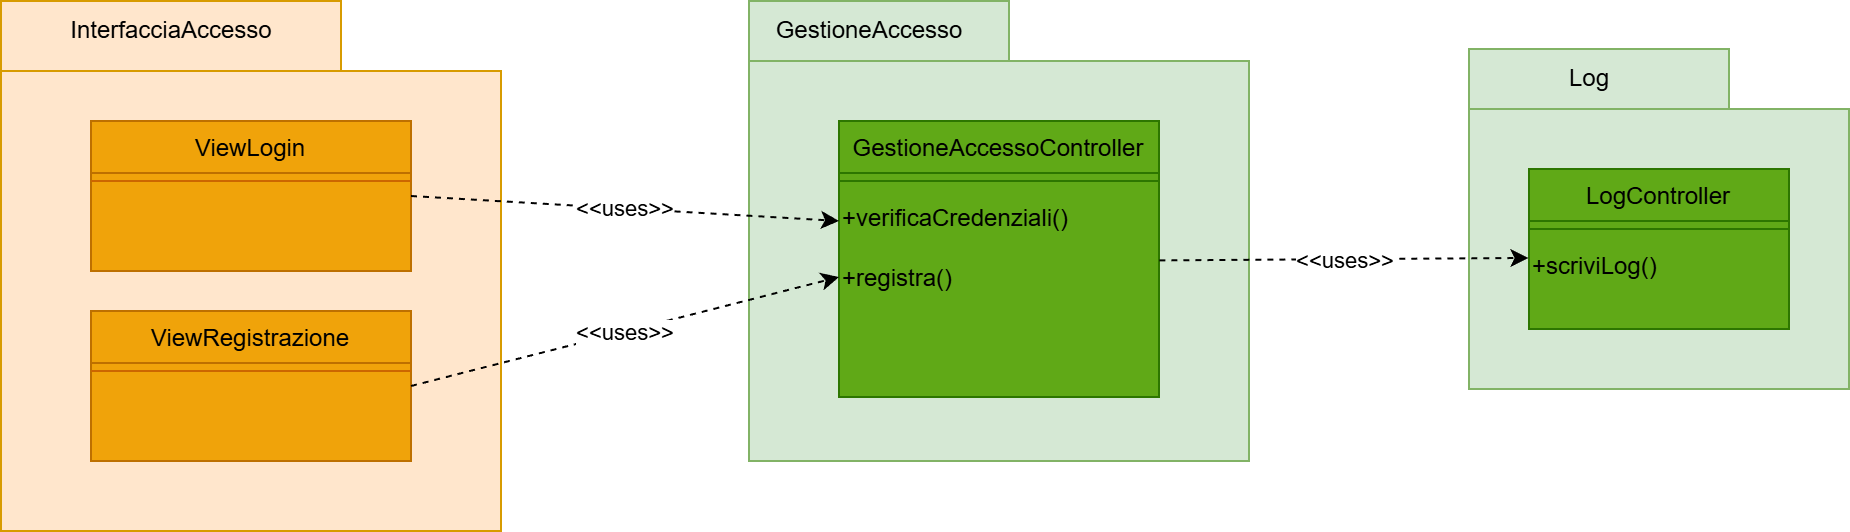
\includegraphics[height=0.18\textheight]{GestioneAccesso.png}
        \caption{Diagramma delle classi: interfacca e gestione accesso}
    \end{center}
\end{figure}



\clearpage